\section{Models}
\label{sec:model-and-main-results}
We start by specifying the high-level SDN programs and low-level datapath models. Since the main focus of SDN is routing, we refer to a high-level SDN program as a routing function. Since multi-table pipelines are the state-of-art for SDN datapaths, we focus on pipelines as datapaths.

\subsection{Routing Function Model}
\label{subsec:function-model}
\para{Routing function:} We denote a routing function as $f$, and assume that it is a logically centralized, deterministic function written in a high level language logically executed by an SDN controller on every packet~\cite{maple} entering that controller's network to determine network-wide routing for that packet.

Each execution of $f$ on a packet reads a set of the packet's attributes (called match fields) $\mathcal{M} = \langle m_1, ..., m_n \rangle$ (\eg, \texttt{<srcIP, dstIP, ...>}). We use $M$ to denote a subset of packet match fields included in $\mathcal{M}$. Moreover, we denote $dom(M)$ as the domain of a set of match fields $M$. The execution of $f$ returns a routing action from a set of valid actions $\mathcal{R}$ (\eg, \texttt{Drop, Forward(port=2)}):

%Any subset of these match fields' $M \in \mathcal{M}$ value $v_i(M)$, however, is restricted to the domain of valid values $dom(M)$ specified by the match fields' headers' network protocols. Given this restriction, $f$ may be summarized as a mapping from values in $f$'s match fields' domain to actions in $\mathcal{R}$:

\begin{equation*}
f : dom(\mathcal{M}) \rightarrow \mathcal{R}.
\end{equation*}

The space of such functions is denoted $\mathcal{F}$.

\para{Example:} We use the routing function \texttt{onPkt} below to illustrate key features of our routing function model.
\begin{verbatim}
\\  Routing function: onPkt
    Map hostTbl[key: dstIP, value: switch]
    Map condTbl[key: (dstIP, port), value: cond]
    Map routeTbl[key: (switch, cond), value: outPort]
L0: onPkt(Type ethType, Addr srcIP, Port srcPort, \
          Addr dstIP, Port dstPort):
L1: if (ethType != IPv4):
L2:   return Drop()
L3: if (verify(srcPort, srcIP)):
L4:   dstCond = condTbl[dstIP, dstPort]
L5:   dstSw = hostTbl[dstIP]
L6:   return Forward(port = routeTbl[dstCond, dstSw])
L7: return Drop()
\end{verbatim}

Specifically, \texttt{onPkt} reads the match fields $\mathcal{M} = \langle \texttt{ethType}, \texttt{srcIP}, \texttt{srcPort}, \texttt{dstIP}, \texttt{dstPort} \rangle$ and maps each value in the domain of $\mathcal{M}$ to a routing action in $\mathcal{R}=\{\texttt{Drop()}, \texttt{Forward(port=x)} \}$. While we write \texttt{onPkt} as an imperative function, we emphasize that our model is fully generic and does not specify a programming paradigm.

Elaborating, \texttt{onPkt}'s first three lines declare key-value tables. Specifically, \texttt{hostTable} and \texttt{condTable} associate each IP address with an attachment switch and host condition (\eg, authentication status) respectively, while \texttt{routeTable} maps a switch, condition pair to its forwarding port. Moving on to \texttt{onPkt}'s body, \texttt{L1} and \texttt{L2} detect and drop non-IPv4 traffic, while \texttt{L7} drops traffic from unverified endpoints. For verified packets, \texttt{L4} to \texttt{L6} further set \texttt{dstCond} and \texttt{dstSw} variables, and then return a routing action  from \texttt{routeTbl} based on the two variables.


\para{Routing function DFG:} Since a generic routing function can have arbitrary, complex control structure, we transform a routing function into a dataflow graph (DFG) to better represent its structure. We denote an $f$'s DFG as $G_f$.

Specifically, to compute $G_f$ for $f$, we must remove all of $f$ control follow dependencies. These dependencies are removed by the following transformations:
\begin{itemize}
  \item We remove assignment statement order dependencies by converting $f$ to single static assignment form (SSA).
  \item We remove branches by assigning their conditionals' values to guards, and appending dependencies on these guards to all statements in their \texttt{if} and \texttt{else} blocks.
  \item We remove program loops by converting them to black box functions which read all variables read by the loop and write all variables written by them.
\end{itemize}

For example, our example routing function \texttt{onPkt} is transformed as follows:

\begin{verbatim}
L0: onPkt(...):
L1: g0 = (ethType != IPv4)
L2: if  g0: return Drop()
L3: g1 = verify(srcPort, srcIP)):
L4: if  g1: dstCond = condTbl[dstIP, dstPort]
L5: if  g1: dstSw = hostTbl[dstIP]
L6: if  g1: return Forward(port = routeTbl[...])
L7: if !g1: return Drop()
\end{verbatim}

Note that \texttt{onPkt}'s \texttt{if} statement at \texttt{L1}'s has been replaced by an assignment from its conditional to the guard \texttt{g0}. This guard is appended to \texttt{L2}, which was formally in the \texttt{if} statement's \texttt{if} block.

Given this transformation, we define $G_f$ for $f$:

\begin{definition} A {\em routing function $f$'s' dataflow graph DFG $G_f = (V_f, E_f)$} is a vertex weighted dag generated from a transformed $f$ such that:
\begin{itemize}
  \item Each vertex $v_f$ in $V_f$ is a variable in $f$.
  \item A $v_f$'s weight is its domain size.
  \item There is a directed edge in $E_f$ between two variables if the source variable appears in the target variable's assignment.
\end{itemize}
\end{definition}

As an example, we give \texttt{onPkt}'s DFG below:
\begin{figure}[tbh]
    \centering
    \vspace{-1mm}
    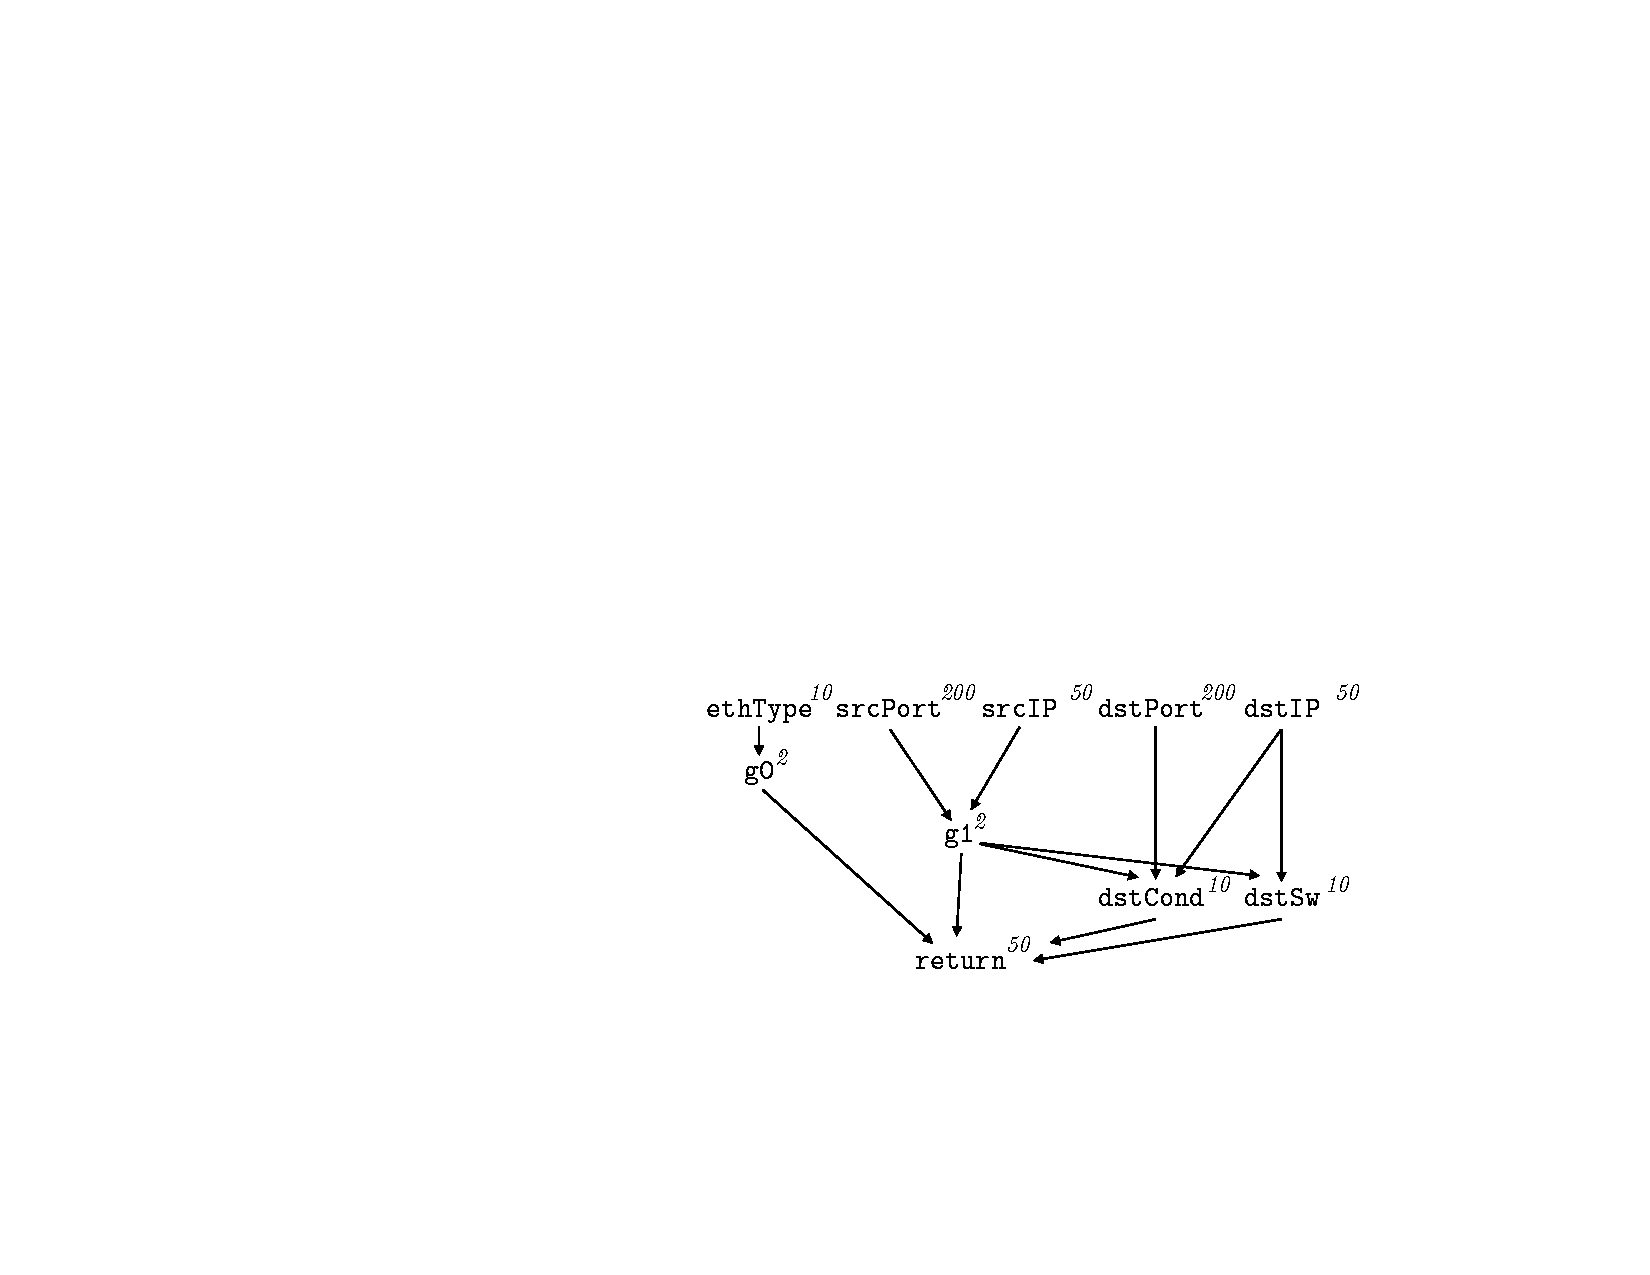
\includegraphics[scale = 0.6]{figures/figure2.pdf}
    \vspace{-2mm}
    \caption{The routing function \texttt{onPkt}'s DFG $G_{\texttt{onPkt}}$.}
    \label{fig:onpkt-dfg}
    \vspace{-2mm}
\end{figure}

Observe that the vertex \texttt{dstSw} is descended from the two variables in its assignment, \texttt{g1} and \texttt{dstIP}. The vertex's weight, $10$, indicates \texttt{dstSw}'s domain.

%IPv4 packets' destination endpoints are mapped to their attachment switch and host condition in \texttt{L4} and \texttt{L5}, which \texttt{L6} uses to look up the packet's next hop forwarding port.

%Elaborating, \texttt{onPkt}'s first three lines declare key-value map state variables. \texttt{hostTable} and \texttt{condTable} associate layer 3 endpoints with their attachment switch and host condition (\eg\ authentication status) respectively while \texttt{routeTable} maps switch condition pairs to their forwarding port. Moving on to \texttt{onPkt}'s body, \texttt{L1} and \texttt{L2} drop non-IPv4 traffic, while \texttt{L3} and \texttt{L7} drop traffic from unverified endpoints. Verified IPv4 packets' destination endpoints are mapped to their attachment switch and host condition in \texttt{L4} and \texttt{L5}, which \texttt{L6} uses to look up the packet's next hop forwarding port.


%\yry{An example function}

%An $f$ specifies such network behavior by conceptually running on every packet entering the network and returning a network routing action for each. We denote  the space of all network routing actions an $f$ can return $\mathcal{R}$, and the space of all $f$  $\mathcal{F}$.

%When a packet enters the network, $f$ reads its header's match fields  $\langle m_1, ..., m_n \rangle$. We denote the set $\forall$ packet match fields $f$ reads $\mathcal{M}$, and subsets of $\mathcal{M}$ $M_i$. Further, we say that the value of a subset of a given packet's header match fields $M_i$ is $v_i(M_i)$. These match fields values are restricted  to the domain of valid values specified by the match fields' header's network protocol, $dom(M_i)$. 

%Given the above, $f$'s type signature is:

\subsection{Pipeline Model}
\label{subsec:pipeline-model}

We focus on state-of-the-art datapaths: multi-table pipelines. We first model a table $t$ in a pipeline $p$ and then we give a clear definition for the pipeline.

%A pipeline $p$ is a singly rooted dag (directed, acyclic graph) of tables $\{t_i\}$. 

\para{Pipeline table:} Each pipeline table $t \in p$ is a exact match match-action table. Each of $t$'s actions is a routing action output, or a write to $t$'s output register $r(t)$ followed by a hop to a subsequent table in $p$, or a simple jump action to a subsequent table in $p$. Not all $t$ output routing actions, and we denote the $t$ that do as an egress table.

Each $t$ matches on a set of inputs $I(t)$ that contains packet match fields $m_i \in \mathcal{M}$ and preceding tables' output registers $r(t)$. Key limitations on a $t$ are the maximum number of rules it can contain and $r(t)$'s bit length, which we denote $maxrules(t)$ and $bits(r(t))$ respectively.

\para{Pipeline:} A pipeline $p$ is a singly rooted dag (directed acyclic graph) of tables $\{t_i\}$. An edge $(t_i, t_j)$ in a $p$ indicates that a packet arriving at $t_i$ can jump to $t_j$. 

%A path $\rho$ in the $p$ is defined as a path from the root table to an egress table in the $p$.

Each packet passing through $p$ starts at $p$'s root and proceeds through $p$ to an egress table. Therefore, each packet passing through $p$ can map to a path in the $p$, along with a routing action for that packet from $\mathcal{R}$. 

A packet's path through $p$ and the action its egress table outputs are determined by the set of packet match fields $\mathcal{M}$ each $t_i \in p$ matches on. Given this, $p$ may also be summarized as a mapping from $dom(\mathcal{M})$ to $\mathcal{R}$, which depends on $p$'s contents.

We denote the space of all pipelines $p$ as $P$.


%\yry{move to next para} that every packet entering the switch is passed through to determine its routing behavior. In $p$'s dag, an edge $(t_i, t_j)$ indicates that \yry{fix} $p$ can jump to $t_j$ after executing $t_i$. We denote the space of all pipelines $p$ as $P$.

%\yry{fix} Each packet passing through $p$ starts at $p$'s root and proceeds through $p$ to an egress table which outputs a routing action for that packet from $\mathcal{R}$. A packet's path through $p$ and the action its egress table outputs are determined by the set of packet match fields $\mathcal{M}$ each $t_i \in p$ matches on. 

%Given this, $p$ may also be summarized as a mapping from $dom(\mathcal{M})$ to $\mathcal{R}$, whose value depends on $p$'s contents. If $p$ has a set of contents which computes an $f$'s mapping from $dom(\mathcal{M})$ to $\mathcal{R}$, $f$ is realizable into $p$, $f \rightrightharpoons p$. \yry{fix}

\begin{figure*}[tbh]
    \centering
    \vspace{-1mm}
    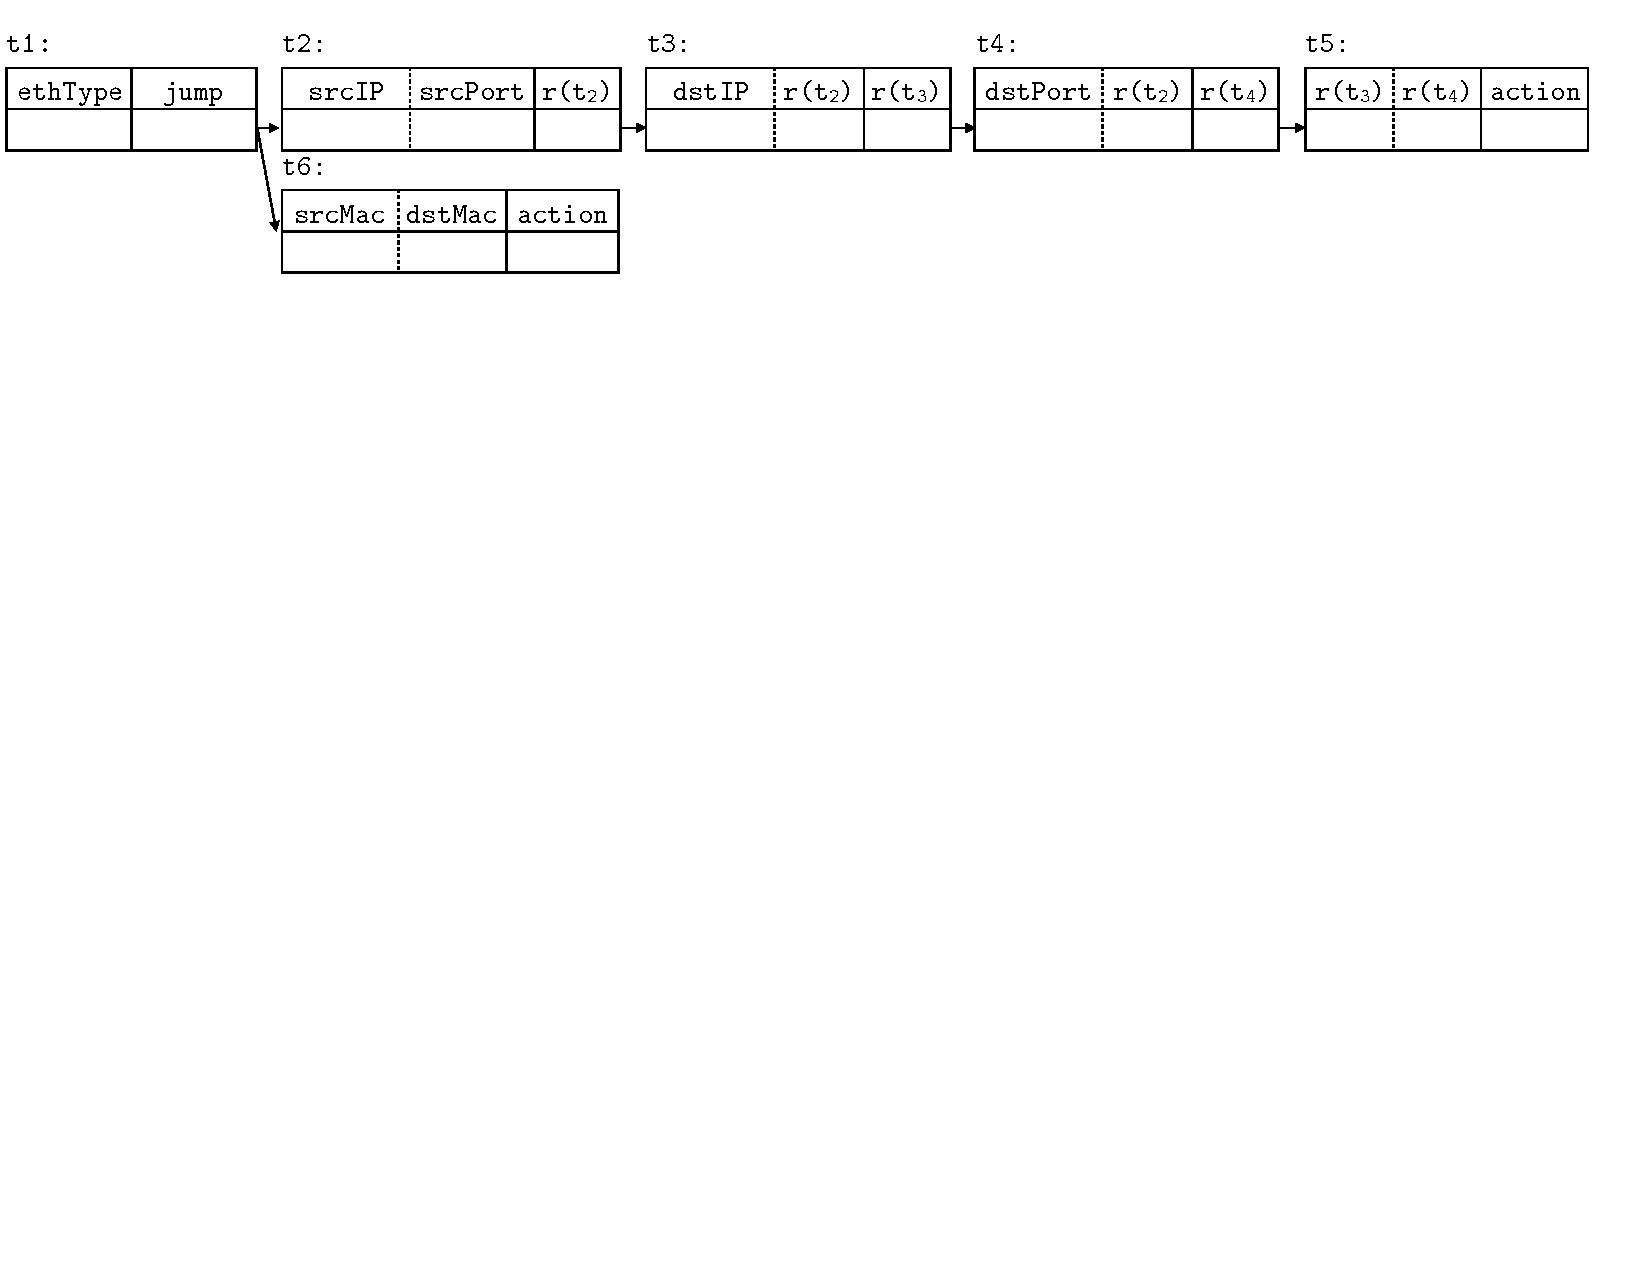
\includegraphics[scale = 0.6]{figures/figure3.pdf}
    \vspace{-2mm}
    \caption{Example datapath, \exampledp}
    \label{fig:swPipeline}
    \vspace{-2mm}
\end{figure*}

\para{Example:} We now give an example pipeline \exampledp, shown in Fig~\ref{fig:swPipeline}, to illustrate our pipeline model. Note that in the example, a table matches on fields on its left-hand side, writes to a register on its right-hand side, and the field \texttt{output} of a table indicates the table contains output routing actions.

%In \exampledp, an incoming packet starts at \exampledp's root \texttt{t1} and is passed to one of \exampledp's two ingress tables \texttt{t5} and \texttt{t6}. Therefore, \exampledp\ contains two paths, $\langle \texttt{t1}, \texttt{t2}, \texttt{t3}, \texttt{t4}, \texttt{t5} \rangle$, and $\langle \texttt{t1}, \texttt{t6} \rangle$.


%The two paths $\rho$ in \texttt{swP} are the paths in its dag from \texttt{t1} to these outputs, $\langle \texttt{t1}, \texttt{t2}, \texttt{t3}, \texttt{t4}, \texttt{t5} \rangle$ and $\langle \texttt{t1}, \texttt{t6} \rangle$.

Narrowing our focus, consider \texttt{t2} $\in$ \exampledp. \texttt{t2} is an exact match table whose inputs $I(\texttt{t2})$ are \texttt{srcIP} and \texttt{srcPort}, and whose output register is \texttt{r(t2)}. %\texttt{t2} is not an egress table and does not output to a pipeline register.

Significant computation limits on \texttt{t2} are its maximum number of rules $maxrules(\texttt{t2}))$ and the size of its output register $bits(\texttt{r(t2)})$.


%Each $t_i$ in \texttt{swP} matches on the fields on its \textit{l.h.s.}, writes to the register on its \textit{r.h.s.}, and can pass control to the $t_j$ its departing edges arrive at. If a $t_i \in$ \texttt{swP} can output routing actions, its \textit{r.h.s.} also contains the field \texttt{output}.



%Consider the structure of \texttt{swP}. \texttt{swP}'s entry table $t_1$ routes incoming traffic to its \texttt{ethType}'s pipeline branch and returns default actions (\eg\ \texttt{Drop()}) for traffic with \texttt{ethType} that \texttt{swP} doesn't handle. $t_2$, $t_3$ and $t_4$ match on L3 packets' headers and perform intermediate processing which $t_5$ uses to compute routing actions. Finally, $t_6$ matches on L2 packets' headers and directly computes their routing actions.

%\yry{A network of switches}
